\documentclass[a4paper,10pt]{article}
\usepackage[utf8]{inputenc}
\usepackage{graphicx}
\usepackage{url}
\usepackage{float}
\usepackage{times}
\usepackage{multirow}
\usepackage{listings}
\usepackage{times}
\usepackage{paralist}
\usepackage{epsfig}
\usepackage{subfigure}
\usepackage[hypertex]{hyperref}
\usepackage{subfigure}
\usepackage{color}
\usepackage{xspace}

%\documentclass{rspublic}

\usepackage{ifpdf}

\newcommand{\I}[1]{\textit{#1}}
\newcommand{\B}[1]{\textbf{#1}}
\newcommand{\BI}[1]{\textbf{\textit{#1}}}
\newcommand{\T}[1]{\texttt{#1}}

\newcommand{\sagaspec}{\textit{SAGA}\xspace}
\newcommand{\sagaimpl}{\textit{SAGA}\xspace}

\newcommand{\spec}{\sagaspec}
\newcommand{\impl}{\sagaimpl}

\setlength\topmargin{0in}
\setlength\headheight{0in}
\setlength\headsep{0in}
\setlength\textheight{9.5in}
\setlength\textwidth{6.5in}
\setlength\oddsidemargin{0in}
\setlength\evensidemargin{0in}
\setlength\parindent{0.1in}
\setlength\parskip{0.25em}


\ifpdf
 \DeclareGraphicsExtensions{.pdf, .jpg}
\else
 \DeclareGraphicsExtensions{.eps, .ps}
\fi

\newcommand{\note}[1]{ {\textcolor{red} { ***NOTE: #1 }}}

\newif\ifdraft
\drafttrue

\ifdraft
\newcommand{\amnote}[1]{   {\textcolor{magenta} { ***Andre:    #1 }}}
\newcommand{\jhanote}[1]{  {\textcolor{red}     { ***Shantenu: #1 }}}
\else
\newcommand{\amnote}[1]{}
\newcommand{\jhanote}[1]{}
\fi

\begin{document}

 \title{ \Large \vspace{-3.5em} Overcoming Infrastructure Barriers on Application Level with SAGA }
 
 \author{Shantenu Jha$^{1,2,3}$, Hartmut Kaiser$^{1}$, Andre Merzky$^{1}$, Ole Weidner$^{1}$ \\
   \small{\emph{$^{1}$Center for Computation \& Technology, Louisiana State University, USA}}\\
   \small{\emph{$^{2}$Department of Computer Science, Louisiana State University, USA}}\\
   \small{\emph{$^{3}$e-Science Institute, University of Edinburgh, UK}}
 }
 \date{}
 \maketitle
 

% \jhanote{Remember in addition to serving as an abstract, this will
%   serve as a summary of what will go to the 3 editors of the journals
%   that we are considering publishing a full paper in. Thus some more
%   information/discussion on what the underlying problem and context
%   will be about.}


% \jhanote{Once we have defined / introduced SAGA, we should probably
%   have 3 subsections -- interface, library and adatptors/backends?}

\subsection*{Introduction}
\vspace{-0.6em}

 Attempts to establish a distributed computing infrastructure ('grid')
 and make it transparently accessible to scientific applications have
 been ongoing for some time. Although some infrastructure providers
 are dedicated to advance the integration of their systems, the very
 idea of a global computing grid, seamless sharing of resources across
 administrative as well as technical domains, is not reality yet. This
 is why still relatively few existing distributed applications exploit
 the full potential of these global distributed environments.
 Especially on the technical side, application developers are facing
 difficulties in their attempt to master the complexity and
 heterogeneity of the underlying infrastructure and the still existing
 barriers between different distributed systems.

 With \impl, the \textit{Simple API for Grid Applications}, we
 introduce a community driven standard and its implementation in
 C++/Python that can help to overcome most of the remaining technical
 barriers in global distributed systems. \impl provides the
 application developer with and extensible, high-level API that
 unifies the access to common grid functionality (job, namespace, file
 and replica handling, streams and RPC). Along with a lightweight
 runtime-system for logging and error handling, and an expanding
 number of middleware \textit{adaptors} (plug-ins to access
 distributed middleware services), \impl provides a simple, yet
 powerful interface to develop portable distributed e-Research applications,
 tools and frameworks that can take full advantage of a growing global
 infrastructure.

\vspace{-0.8em}

\subsection*{A Powerful, Community-Driven Standard}
\vspace{-0.6em}

 The \spec effort was initially triggered by several early grid
 adopter communities, which perceived the need for a simple, uniform,
 and stable programmatic interface for distributed (grid) applications
 that is widely-adopted and widely-available. The distributed
 computing community was looking for something similar to what the
 \textit{Message Passing Interface} (MPI) standard is for the parallel
 computing community -- a ``\textit{grid-counterpart to MPI}'' that
 allows the development of portable distributed applications.
 
 
 The scope and requirements of the \spec API is formally defined by
 the Open Grid Forum's (OGF)~\cite{ogf} SAGA Working Group (SAGA-WG),
 and were derived from use cases collected from a broad user community
 (see GFD.70~\cite{ogf-gfd-70} and GFD.71~\cite{ogf-gfd-71}). The
 result of this 5-year process is the \spec Core API specification 1.0
 (GFD.90~\cite{ogf-gfd-90}) which defines the \spec Core (including
 error handling, session management, monitoring, notification, and
 asynchronous operations) and the \spec \textit{Functional API
 Packages} (jobs, namespaces, files, replicas, streams, RPC).
 Additional API extension packages, such as Checkpoint \& Recovery
 (CPR) (GWD-R.96~\cite{ogf-gwd-r-96}), Adverts
 (GFD-R-P.XX~\cite{ogf-gwd-r-p-xx}), and Messaging
 (GWD-R.94~\cite{ogf-gwd-r-94}) are currently under development and
 follow a similar, well-defined community-driven standardization and
 approval process. 

 
 The \spec interface follows a clean class-based object-oriented
 design paradigm and is formulated in an abstract way (using SIDL)
 which allows implementations of the standard in most object-oriented
 and even procedural programming languages. GFD.90 is now an Open Grid
 Forum proposed recommendation on the path to becoming a full standard
 in 2010. \spec is probably the most advanced and also most complete
 attempt and to create a standard that defines a unified programming
 interface for the distributed-application community - something the
 parallel-application community has benefited from for the past 16
 years since the release of the MPI 1.0 standard in 1994. 
 
\vspace{-0.8em}


\subsection*{A Modular and Extensible C++ / Python Implementation}
\vspace{-0.6em}

 Along with the evolution of the \spec standard, our group developed a
 \impl reference implementation using the C++ and Python programming
 languages. Initially started as a proof-of-concept and to ensure the
 implementability of the standard, our \impl implementation has
 evolved into a stable and widely-used production-level software
 library -- with extensive support for commonly used distributed grid
 middleware.  It implements the \spec \textit{Core} and
 \textit{Functional Packages} (GFD.90~\cite{ogf-gfd-90}) as well as
 experimental packages for \textit{Adverts}~\cite{ogf-gwd-r-p-xx},
 \textit{Messaging}\cite{ogf-gwd-r-94} and
 \textit{CPR}~\cite{ogf-gwd-r-96} as a set of independent dynamic
 libraries. \impl is Open Source software, released under the Boost
 Software License 1.0~\cite{boost_license_web}. 

 With flexibility and extensibility as one of its main design goals,
 \impl's structure is highly modular. It can be divided into four
 major components as depicted in Fig. \ref{fig:saga_arch} (left): (1)
 the \I{Core} which implements a lightweight runtime system, (2) the
 \I{Functional Packages} providing the actual Grid API methods, (3)
 the Python API \I{Language Bindings} -- a thin wrapper layer on top
 of the native C++ interface, and (4) the \I{Adaptors} (plug-ins)
 which translate calls from the \I{Functional Packages} API into
 native middleware calls.  The runtime-system is capable of loading
 \I{Adaptors} (also realized as dynamic libraries) at runtime and
 dispatch the API calls to those \I{Adaptors} that are capable of
 executing them on a specific grid middleware [Fig.
 \ref{fig:saga_arch} (right)]. Each \I{Adaptor} implements the
 functionality of a specific functional package (e.g., job adaptors,
 file adaptors) for a specific middleware system. \impl provides
 support for a plethora grid and distributed computing middleware,
 including the Globus Toolkit, Condor, Platform LSF, GridSAM, SSH and
 Amazon EC2. Several other adaptors, notably adaptors for PBS,
 gLite-CREM and BES/Unicore are under development. 

 The layered, decoupled architecture of \impl allows for maximum
 flexibility at compile and runtime. It allows the user of to freely
 and selectively combine the library components and easily develop
 additional components orthogonal to the existing ones (e.g., a new
 functional package APIs). The exclusive use of the PIMPL idiom
 (pointer to implementation) makes the SAGA API objects very
 lightweight and allows a clean separation between the fa\c{c}ade
 (API) and the implementation (CPI/Adaptors). A pleasant side-effect
 of this design decision is the absence of pointers and references in
 the \impl C++ API.

%  The forth and last
% component are the \I{Command Line Tools}. They provide a
% non-programmatic access to each of \impl's functional packages: the
% \I{file tool} provides access to file operations, like read, copy,
% delete, move, etc., the \textit{job tool} allows simple submission and
% control ofcompute jobs, and so on.
\vspace{-0.8em}


\subsection*{A Mature Software Engineering Process\label{engineering}}
\vspace{-0.6em}

 Over the last three years of \impl development, our group has apprehended 
 that besides having an appropriate and scalable system architecture, the main challenge in
 creating sustainable and good quality tools and software systems lies 
 in the software engineering process. The \impl engineering process follows an iterative and incremental
 model in which the evaluation and learning phase is strongly
 community driven, and is closely supervised by the technical project
 manager.  \impl provides independent releases for the \I{Core
 Components}, the \I{Language Bindings} and the \I{Adaptors}, which
 provides maximum flexibility and short reaction times for
 bugfix-releases. All releases are available on the \impl
 website~\cite{saga_downloads_web} and are fed into a very responsive
 community of users, which subsequently files bugs and suggests
 improvement through a central ticket
 system~\cite{saga_bugtracking_web} which is tightly integrated into
 the development process. These reports along with strategic long-term
 development goals form the requirements for the next iteration.
 Individual developers are usually responsible for specific components
 over the component's whole lifetime. This does not only ensure
 clearly defined targets for task assignments, but also results in
 growing expertise and specialization for the individual developers.
 The core \impl development team has been working together for more
 than three years and has evolved into a very smooth running
 operation.  Nevertheless, the \impl development process is completely
 open: community involvement is not only accepted but encouraged and
 has lead to successful collaborations and enrichment of the \impl
 landscape in the past.

 Along with the development of \impl, we maintain and constantly
 extend a broad set of unit and conformance tests to verify proper
 functioning and to validate OGF standard compliance. Most of the
 tests are written on a per-package basis using the Boost Test
 library~\cite{boost_test_web} and Python's built-in unit test
 framework. To facilitate the continuous integration (CI) aspect in
 the \impl development process, all tests are run constantly and
 automated using an automated CI rig\cite{buildbot_web} which provides
 feedback for every single change in the \impl source tree. This way
 build problems and failing tests are pinpointed quickly and the
 responsible developer can take action. These automated tests are  our
 most valuable tool for early error and bug detection and has lead to
 a constantly higher quality of our releases since its introduction.

\vspace{-0.8em}
%\subsection*{A Strong and Diverse Application Community}

\subsection*{Addressing the Needs of the e-Science Community}
\vspace{-0.6em}
%\jhanote{SJ Will write} \note{Shantenu's playground: talk about
%  scientific applications using saga directly (...), talk about CS
%  people taking saga and use it to build higher-level frameworks and
%  tools (faust, bigjob, diggedag...). The usual stuff ;-)}

 \impl is being used by a broad set of users in many different ways -- both to
 support production-grade science as well as to facilitate research into
 distributed systems and applications.  For applications, the most common mode
 of uptake has been in the development of ``frameworks'' -- logical compoments
 that meet specific application requirements. Some specific examples of such
 frameworks include the Pilot-Job Framework (BigJob) and a self-adapting
 computing framework (Lazarus); other frameworks are based upon generalisations
 of well known patterns such as All-Pairs or MapReduce.  SAGA-based frameworks
 support a wide-range of scientific activity, ranging from the Virtual
 Physiological Human (VPH) to resorvoir simulations and hierarchichal molecular
 dynamics simulations on the TeraGrid.

 Another common mode of SAGA usage is the creation of tools that are
 extensible and work over different infrastructure. Once again,
 SAGA-based tools are being utilised for production-grade as well as
 research-prototyping. Prominent examples of the former, include the
 GANGA-DIANE toolset, JSAGA, NAREGI job submission/management system.
 Examples of research prototypes include digedags -- an experimental
 system to support the flexible execution of DAG-based workflow
 applications.

 Finally, several applications (e.g., numerical relativity
 applications) have used SAGA directly to support remote job
 submission and file/date transfer. Although this was an initial
 target usage mode, the cumulative number of such users is less than
 the previous two modes. It is worth mentioning that applications
 typically tend to use \impl directly in early (fast-track) stages, but
 then move to deeper integration via \impl-based frameworks.  \vspace{-0.8em}
 \pagebreak

\begin{figure}%[hb]
  \centering
  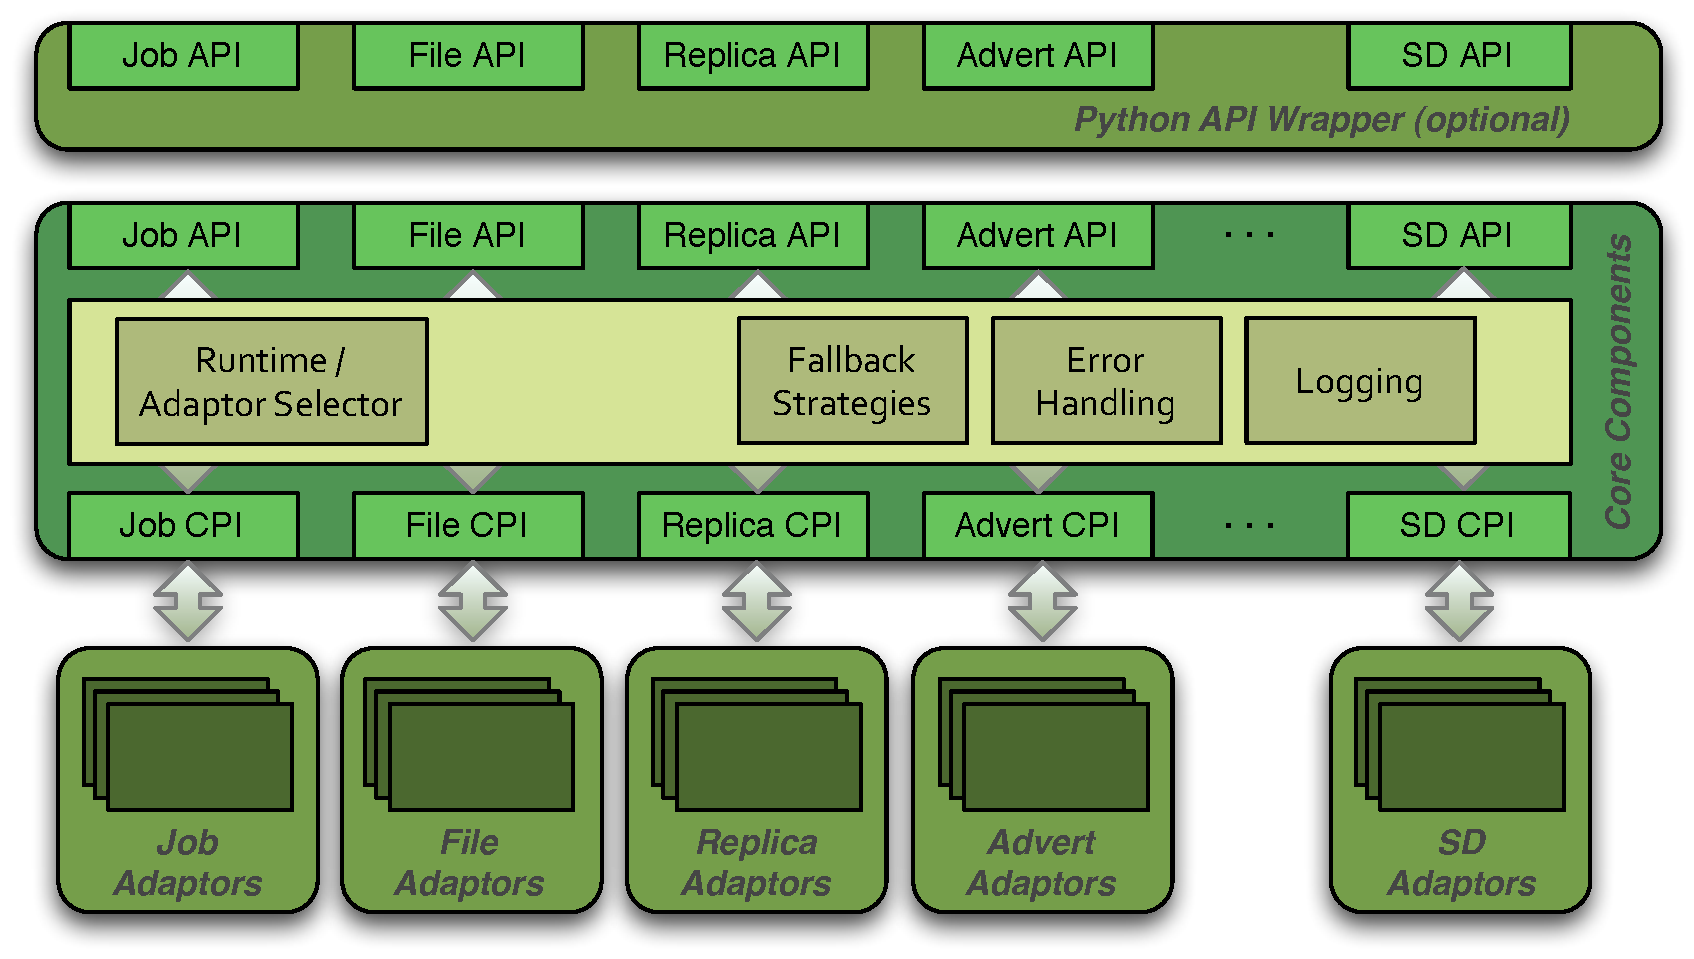
\includegraphics[width=3.23in]{./figures/saga-architecture}
  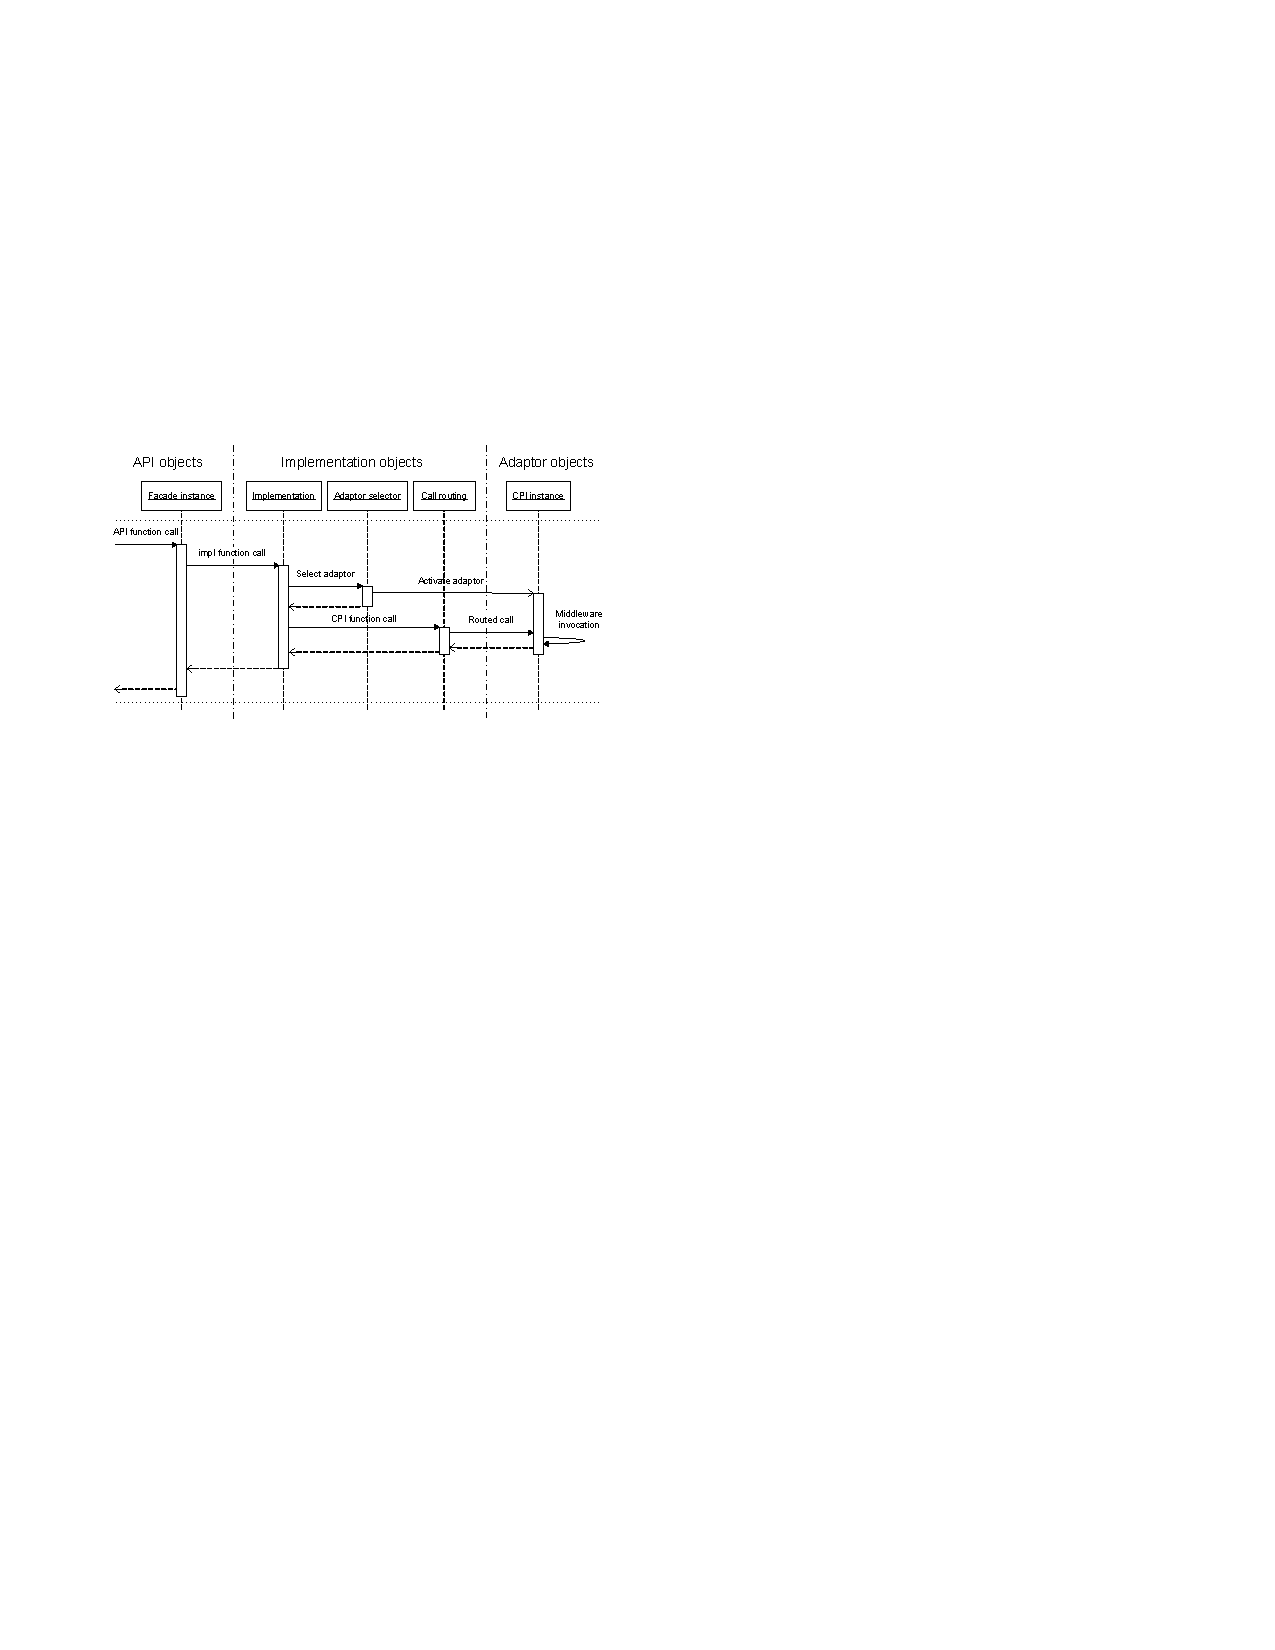
\includegraphics[width=3.23in]{./figures/saga-call-dispatch}

 \vspace{-1em}	
  \caption{\footnotesize \B{Left:} Layered schematic of the modular
  and extensible architecture of \impl. A lightweight runtime
  dispatches API calls to a set of middleware adaptors (plug-ins). An
  optional Python API wrapper adds Python scripting support to SAGA.
  \B{Right: } Sequence-diagram showing the execution sequence through
  the different object instances for any SAGA API call: The fa\c{c}ade
  object calls the internal (private) implementation object which
  triggers the dynamic adaptor selection mechanism. Once an adaptor is
  found, the implementation object calls the appropriate adaptor
  method, which tries to execute the call on the middleware. }
    
%\vspace{-1.5em}
  \label{fig:saga_arch}
\end{figure}


 \bibliographystyle{IEEEtran} 
 \bibliography{saga_ahm_abstract,saga_ogf}


\end{document}

